\section{UserCSP Design}
\label{sec:design}

The goal of our approach, UserCSP, is to help web site
administrators and website users to write comprehensive
CSP rules for the website.

\begin{figure}[h!]
\center
  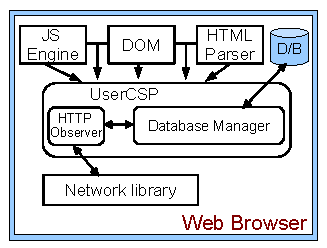
\includegraphics{userCSP_Arch}
\caption{UserCSP Architecture}
\label{fig:userCSP-Arch}
\end{figure}

Figure~\ref{fig:userCSP-Arch} illustrates the architecture of
UserCSP. To enforce user specified Content Security Policy as well as
to infer CSP policy for a website, UserCSP monitors web browsers
internal events including HTML parsing, HTTP requests, XHR, etc., and
analyzes the type of content loaded by a web page and source of that
content. Database manager component of the UserCSP is responsible for
storing user specified CSP rules for websites into local database and
retrieves the corresponding CSP rules for the website when user loads
the website.

When users visits a website, UserCSP performs one of
the following actions:


\begin{itemize}

\item If website has defined CSP, but the user hasn��t specified a CSP
  policy for that website, then UserCSP doesn��t interfere with the
  website defined CSP rules.  However, it allows the user the option
  to amend the website's CSP.

\item If a user has specified CSP rules for a website, but the website
  administrators hasn��t defined a CSP for their website, then the user
  specified CSP policy will be enforced by the UserCSP.
 
\item If a user specified CSP exists as well as a website defined CSP,
  then users have a choice either to apply their own policy or adopt
  the website defined policy. Moreover, users can also select a strict
  or loose set of CSP rules by combining their own policy with the
  website defined policy. For example, if a website sets ��script-src
  www.example.com;�� and user specifies ��script-src www.example.com
  www.abc.com;�� then the strict policy would be ��script-src
  www.example.com;�� whereas the loose policy would be ��script-src
  www.example.com www.abc.com;��.

\item If neither user nor website administrators specifiy a CSP for a
  website then UserCSP doesn��t interfere with the content loading on
  the website.

\item To allow automatic inference of a CSP for websites, UserCSP
  monitors content loaded by web pages and recommends CSP rules based
  on the types of content and sources of that content. It also
  monitors the resources dynamically added to the web page by
  JavaScript.

\end{itemize}
